% !TeX root = ../tfg.tex
% !TeX encoding = utf8
%
% ====================================================================
%  CAPÍTULO 1 — INTRODUCCIÓN DE LA EMPRESA Y ORGANIGRAMA
%
%  RECORDATORIO AL EQUIPO:
%  Este capítulo sitúa al lector. Debe incluir:
%    - Descripción breve pero completa: sector, tamaño, historia reciente,
%      presencia geográfica, número de empleados, cifras clave.
%    - El organigrama: niveles jerárquicos, áreas funcionales y, si es
%      posible, el departamento de RRHH destacado.
%    - Cómo está estructurada la empresa formalmente vs. cómo funciona
%      realmente (funcional, divisional o matricial).
%    - Si tenéis el organigrama como imagen, guardadla en /img/
%      y usad \includegraphics. Si no, describidlo en texto.
%  Fuentes útiles: Memoria Anual CaixaBank, CNMV, web corporativa.
% ====================================================================

\chapter{La empresa: CaixaBank}

% ============================================================
\section{Descripción general}
% ============================================================

% TODO: Ampliad con datos reales obtenidos de la entrevista y fuentes
% oficiales (Memoria Anual CaixaBank, CNMV, web corporativa).
% Actualizad las cifras si han variado desde las que figuran aquí.

CaixaBank, S.A. es una entidad bancaria española con sede central en Valencia.
Surgida de la reorganización del Grupo ``la Caixa'', cotiza en el IBEX~35
y es actualmente uno de los mayores grupos financieros de España y Portugal
tras la fusión con Bankia completada en 2021.

\begin{table}[H]
  \centering
  \caption{Datos corporativos básicos de CaixaBank}
  \begin{tabularx}{\textwidth}{lX}
    \toprule
    \textbf{Parámetro}           & \textbf{Valor} \\
    \midrule
    Sector                       & Servicios financieros y bancarios \\
    Año de fundación             & 1904 (origen en Caja de Pensiones para la Vejez y de Ahorros) \\
    Sede central                 & Valencia, España \\
    Número de empleados          & $\sim$45.000 (grupo consolidado, 2024) \\
    Número de oficinas           & $\sim$4.000 en España \\
    Presencia internacional      & Portugal (BPI), Luxemburgo, Reino Unido, entre otros \\
    Cotización                   & IBEX~35 (ticker: CABK) \\
    Facturación / Margen bruto   & [Dato real a incluir] \\
    \bottomrule
  \end{tabularx}
\end{table}

% ============================================================
\section{Organigrama}
% ============================================================

% ------------------------------------------------------------------
%  COLORES PARA EL ORGANIGRAMA (tonos rojo plantilla UGR)
% ------------------------------------------------------------------
\definecolor{cCEO} {rgb}{0.40,0.02,0.02}
\definecolor{cL1}  {rgb}{0.58,0.07,0.07}
\definecolor{cGr}  {HTML}{155934}
\definecolor{cGr2} {HTML}{277048}
\definecolor{cEmp} {HTML}{7A8694}
\definecolor{cCard}{HTML}{FFFFFF}
\definecolor{cBord}{rgb}{0.80,0.68,0.68}
\definecolor{cConn}{rgb}{0.68,0.52,0.52}
\definecolor{cDark}{HTML}{1A0A0A}
\definecolor{cGray}{HTML}{5C4A4A}
\definecolor{cBg}  {rgb}{0.98,0.95,0.95}

% \nc{left_x}{top_y}{color}{titulo}{subtitulo}
\newcommand{\nc}[5]{%
  \fill[black!8,rounded corners=2.5pt](#1+.07,{-(#2)-.07})rectangle(#1+2.94+.07,{-(#2)-2.20-.07});
  \fill[cCard,rounded corners=2.5pt,draw=cBord,line width=.35pt](#1,{-(#2)})rectangle(#1+2.94,{-(#2)-2.20});
  \fill[#3,rounded corners=2.5pt](#1,{-(#2)})rectangle(#1+2.94,{-(#2)-.22});
  \fill[#3](#1,{-(#2)-.11})rectangle(#1+2.94,{-(#2)-.22});
  \fill[#3!22,draw=#3!55,line width=.4pt](#1+.26,{-(#2)-.58})circle(.22);
  \node[anchor=north west,text width=2.32cm,inner sep=0pt,align=left,
        font=\fontsize{5.5}{6.5}\bfseries\sffamily\selectfont,text=cDark]
    at(#1+.54,{-(#2)-.28}){#4};
  \def\tmpS{#5}\ifx\tmpS\empty\else
  \node[anchor=south west,text width=2.78cm,inner sep=0pt,align=left,
        font=\fontsize{4.6}{5.4}\sffamily\selectfont,text=cGray]
    at(#1+.08,{-(#2)-2.10}){#5};\fi}

\newcommand{\vc}[3]{\draw[cConn,line width=.5pt](#1,{-(#2)})--(#1,{-(#3)});}

\begin{sidewaysfigure}[p]
  \centering
  \scalebox{0.65}{%
  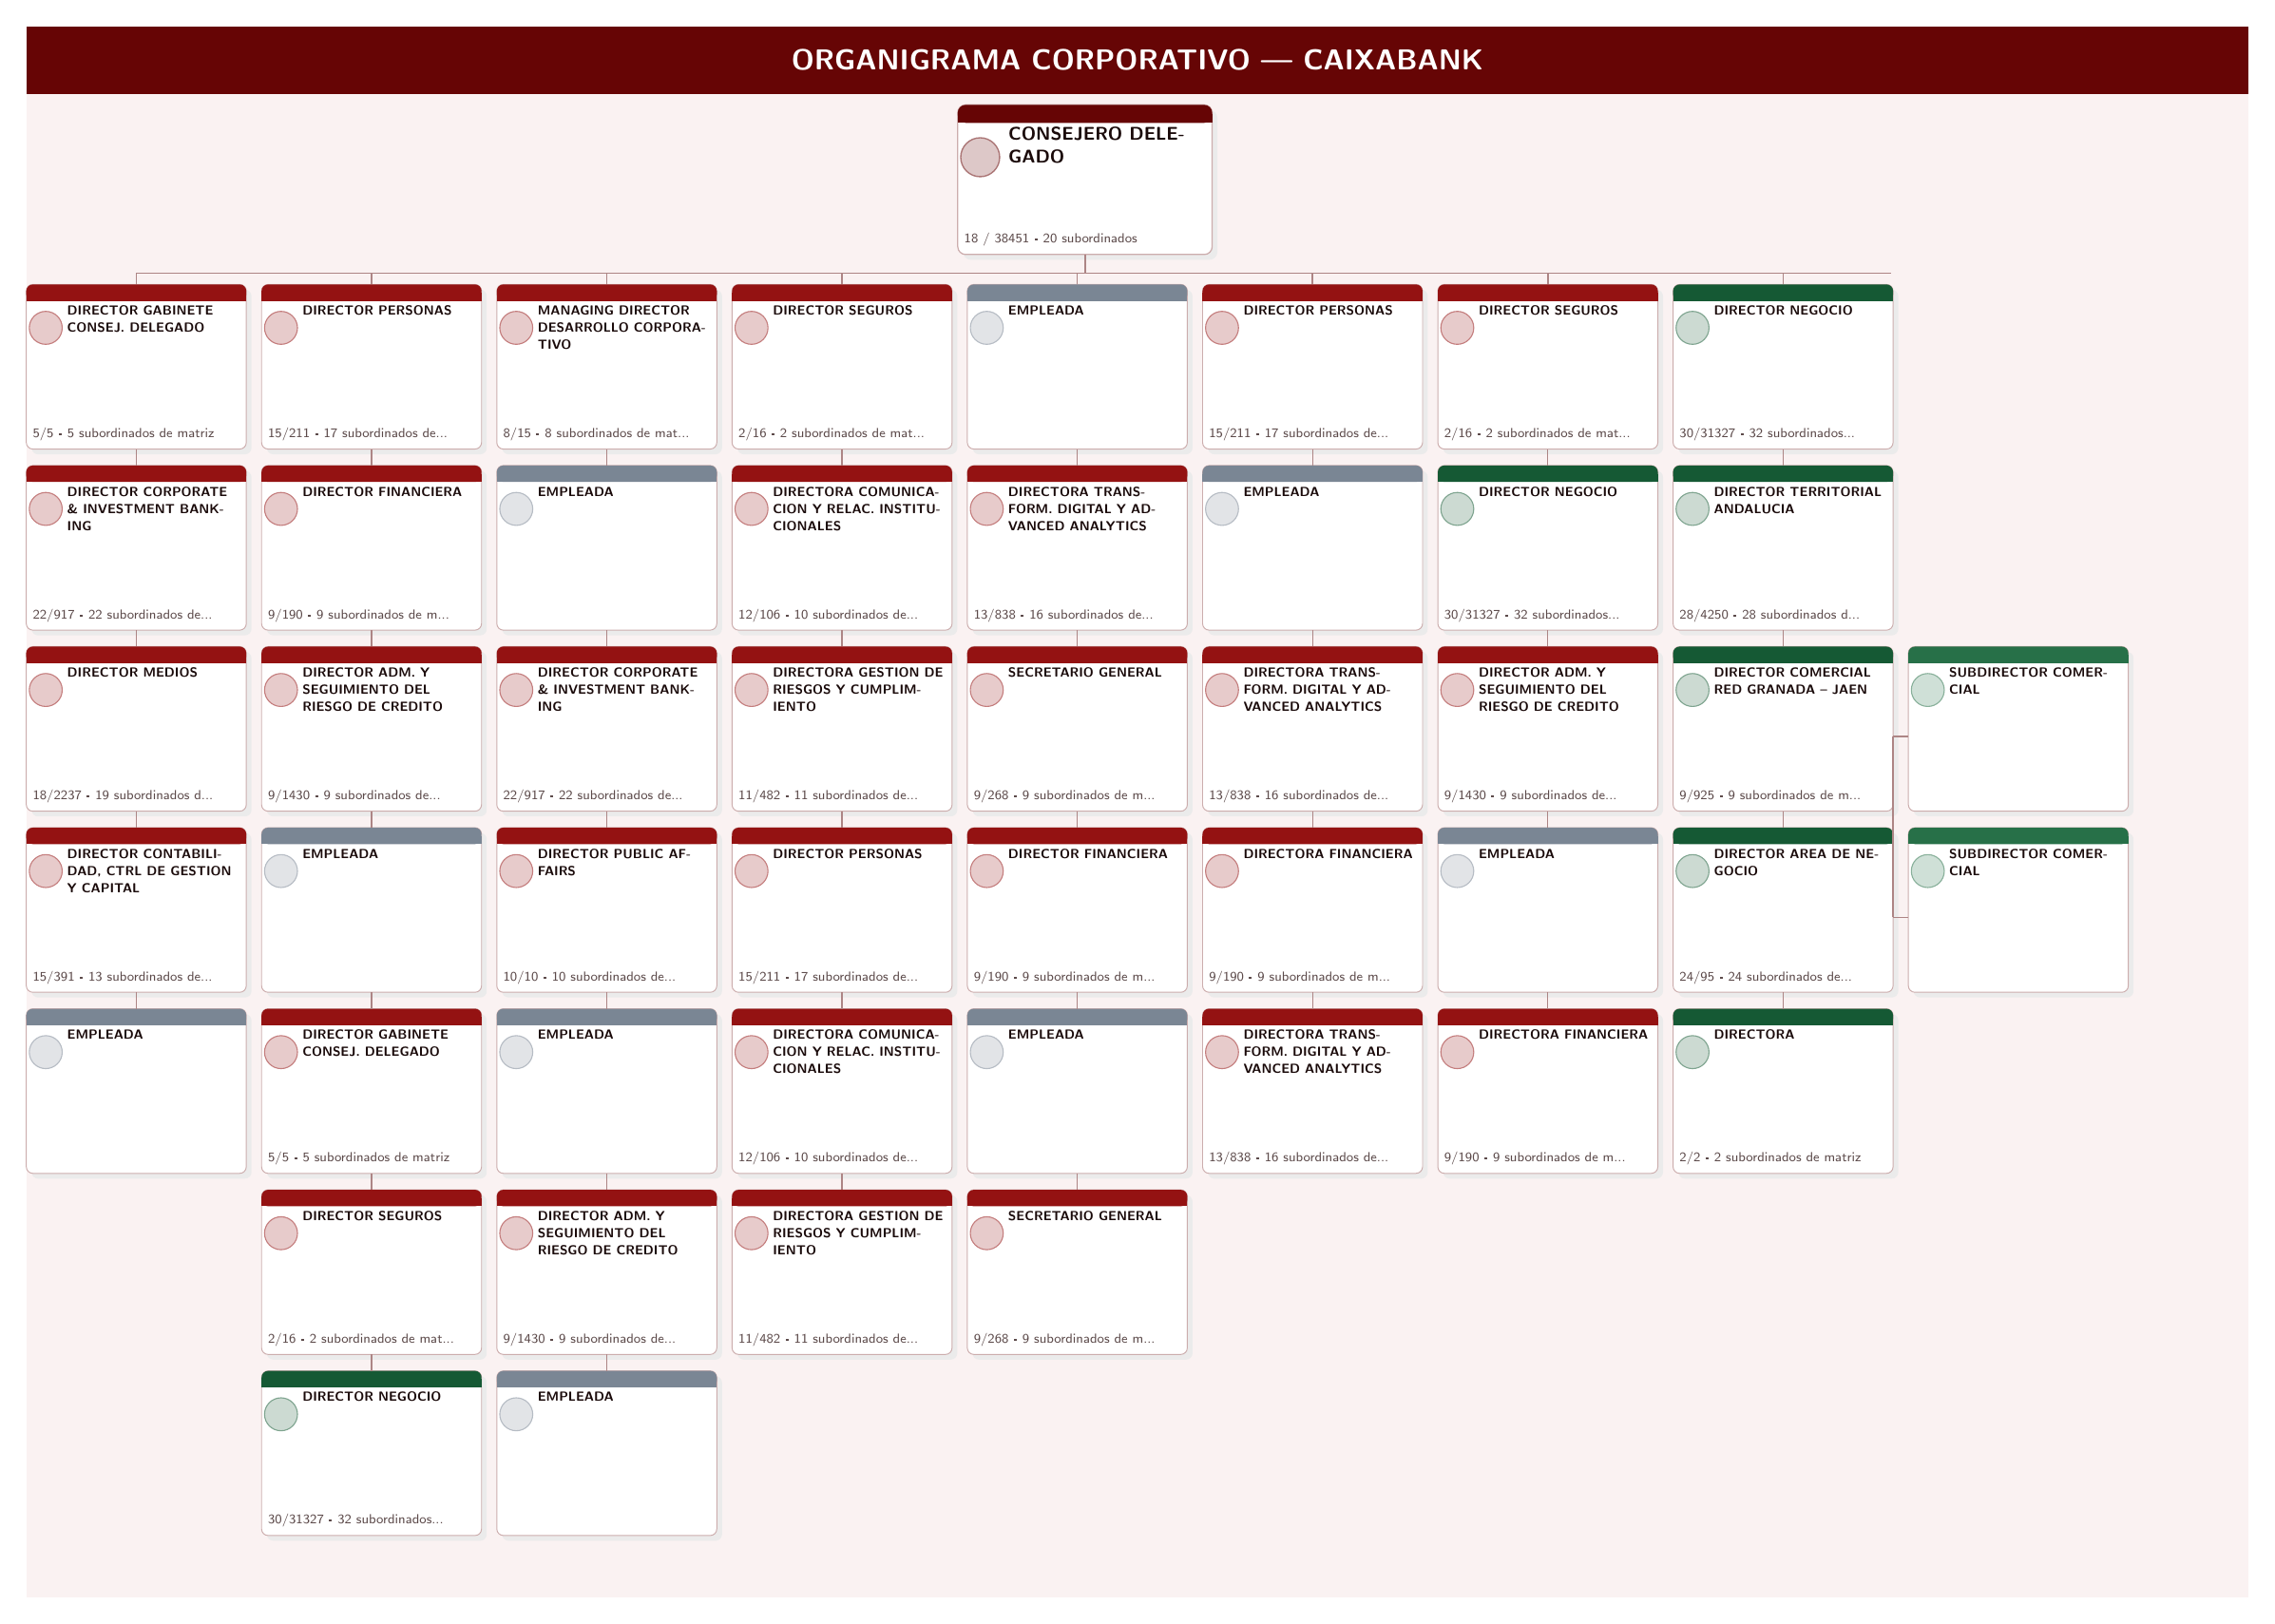
\begin{tikzpicture}[x=1cm,y=1cm,trim left=0cm]

    %% Fondo y barra título (A4 landscape = 29.7 x 21.0 cm)
    \fill[cBg](0,0)rectangle(29.7,-21.0);
    \fill[cCEO](0,0)rectangle(29.7,-.90);
    \node[text=white,font=\fontsize{10.5}{12}\bfseries\sffamily\selectfont,anchor=center]
      at(14.85,-.45){ORGANIGRAMA CORPORATIVO — CAIXABANK};

    %% CEO (centrado)
    \fill[black!8,rounded corners=3pt](12.518,-1.12)rectangle(15.918,-3.12);
    \fill[cCard,rounded corners=3pt,draw=cBord,line width=.45pt](12.448,-1.05)rectangle(15.848,-3.05);
    \fill[cCEO,rounded corners=3pt](12.448,-1.05)rectangle(15.848,-1.29);
    \fill[cCEO](12.448,-1.17)rectangle(15.848,-1.29);
    \fill[cCEO!22,draw=cCEO!55,line width=.5pt](12.748,-1.75)circle(.26);
    \node[anchor=north west,text width=2.86cm,inner sep=0pt,align=left,
          font=\fontsize{7}{8.5}\bfseries\sffamily\selectfont,text=cDark]
      at(13.118,-1.35){CONSEJERO DELEGADO};
    \node[anchor=south west,text width=3.22cm,inner sep=0pt,align=left,
          font=\fontsize{5.2}{6}\sffamily\selectfont,text=cGray]
      at(12.528,-2.95){18 / 38451 · 20 subordinados};

    %% Conectores CEO -> grilla
    \draw[cConn,line width=.6pt](14.148,-3.05)--(14.148,-3.30);
    \draw[cConn,line width=.6pt](1.47,-3.30)--(24.918,-3.30);
    \foreach \cx in {1.47,4.614,7.758,10.902,14.046,17.190,20.334,23.478}{
      \draw[cConn,line width=.55pt](\cx,-3.30)--(\cx,-3.45);}

    %% FILA 1
    \nc{0.000}{3.45}{cL1}{DIRECTOR GABINETE CONSEJ. DELEGADO}{5/5 · 5 subordinados de matriz}
    \nc{3.144}{3.45}{cL1}{DIRECTOR PERSONAS}{15/211 · 17 subordinados de...}
    \nc{6.288}{3.45}{cL1}{MANAGING DIRECTOR DESARROLLO CORPORATIVO}{8/15 · 8 subordinados de mat...}
    \nc{9.432}{3.45}{cL1}{DIRECTOR SEGUROS}{2/16 · 2 subordinados de mat...}
    \nc{12.576}{3.45}{cEmp}{EMPLEADA}{}
    \nc{15.720}{3.45}{cL1}{DIRECTOR PERSONAS}{15/211 · 17 subordinados de...}
    \nc{18.864}{3.45}{cL1}{DIRECTOR SEGUROS}{2/16 · 2 subordinados de mat...}
    \nc{22.008}{3.45}{cGr}{DIRECTOR NEGOCIO}{30/31327 · 32 subordinados...}
    %% FILA 2
    \nc{0.000}{5.87}{cL1}{DIRECTOR CORPORATE \& INVESTMENT BANKING}{22/917 · 22 subordinados de...}
    \nc{3.144}{5.87}{cL1}{DIRECTOR FINANCIERA}{9/190 · 9 subordinados de m...}
    \nc{6.288}{5.87}{cEmp}{EMPLEADA}{}
    \nc{9.432}{5.87}{cL1}{DIRECTORA COMUNICACION Y RELAC. INSTITUCIONALES}{12/106 · 10 subordinados de...}
    \nc{12.576}{5.87}{cL1}{DIRECTORA TRANSFORM. DIGITAL Y ADVANCED ANALYTICS}{13/838 · 16 subordinados de...}
    \nc{15.720}{5.87}{cEmp}{EMPLEADA}{}
    \nc{18.864}{5.87}{cGr}{DIRECTOR NEGOCIO}{30/31327 · 32 subordinados...}
    \nc{22.008}{5.87}{cGr}{DIRECTOR TERRITORIAL ANDALUCIA}{28/4250 · 28 subordinados d...}
    %% FILA 3
    \nc{0.000}{8.29}{cL1}{DIRECTOR MEDIOS}{18/2237 · 19 subordinados d...}
    \nc{3.144}{8.29}{cL1}{DIRECTOR ADM. Y SEGUIMIENTO DEL RIESGO DE CREDITO}{9/1430 · 9 subordinados de...}
    \nc{6.288}{8.29}{cL1}{DIRECTOR CORPORATE \& INVESTMENT BANKING}{22/917 · 22 subordinados de...}
    \nc{9.432}{8.29}{cL1}{DIRECTORA GESTION DE RIESGOS Y CUMPLIMIENTO}{11/482 · 11 subordinados de...}
    \nc{12.576}{8.29}{cL1}{SECRETARIO GENERAL}{9/268 · 9 subordinados de m...}
    \nc{15.720}{8.29}{cL1}{DIRECTORA TRANSFORM. DIGITAL Y ADVANCED ANALYTICS}{13/838 · 16 subordinados de...}
    \nc{18.864}{8.29}{cL1}{DIRECTOR ADM. Y SEGUIMIENTO DEL RIESGO DE CREDITO}{9/1430 · 9 subordinados de...}
    \nc{22.008}{8.29}{cGr}{DIRECTOR COMERCIAL RED GRANADA -- JAEN}{9/925 · 9 subordinados de m...}
    \nc{25.152}{8.29}{cGr2}{SUBDIRECTOR COMERCIAL}{}
    %% FILA 4
    \nc{0.000}{10.71}{cL1}{DIRECTOR CONTABILIDAD, CTRL DE GESTION Y CAPITAL}{15/391 · 13 subordinados de...}
    \nc{3.144}{10.71}{cEmp}{EMPLEADA}{}
    \nc{6.288}{10.71}{cL1}{DIRECTOR PUBLIC AFFAIRS}{10/10 · 10 subordinados de...}
    \nc{9.432}{10.71}{cL1}{DIRECTOR PERSONAS}{15/211 · 17 subordinados de...}
    \nc{12.576}{10.71}{cL1}{DIRECTOR FINANCIERA}{9/190 · 9 subordinados de m...}
    \nc{15.720}{10.71}{cL1}{DIRECTORA FINANCIERA}{9/190 · 9 subordinados de m...}
    \nc{18.864}{10.71}{cEmp}{EMPLEADA}{}
    \nc{22.008}{10.71}{cGr}{DIRECTOR AREA DE NEGOCIO}{24/95 · 24 subordinados de...}
    \nc{25.152}{10.71}{cGr2}{SUBDIRECTOR COMERCIAL}{}
    %% FILA 5
    \nc{0.000}{13.13}{cEmp}{EMPLEADA}{}
    \nc{3.144}{13.13}{cL1}{DIRECTOR GABINETE CONSEJ. DELEGADO}{5/5 · 5 subordinados de matriz}
    \nc{6.288}{13.13}{cEmp}{EMPLEADA}{}
    \nc{9.432}{13.13}{cL1}{DIRECTORA COMUNICACION Y RELAC. INSTITUCIONALES}{12/106 · 10 subordinados de...}
    \nc{12.576}{13.13}{cEmp}{EMPLEADA}{}
    \nc{15.720}{13.13}{cL1}{DIRECTORA TRANSFORM. DIGITAL Y ADVANCED ANALYTICS}{13/838 · 16 subordinados de...}
    \nc{18.864}{13.13}{cL1}{DIRECTORA FINANCIERA}{9/190 · 9 subordinados de m...}
    \nc{22.008}{13.13}{cGr}{DIRECTORA}{2/2 · 2 subordinados de matriz}
    %% FILA 6
    \nc{3.144}{15.55}{cL1}{DIRECTOR SEGUROS}{2/16 · 2 subordinados de mat...}
    \nc{6.288}{15.55}{cL1}{DIRECTOR ADM. Y SEGUIMIENTO DEL RIESGO DE CREDITO}{9/1430 · 9 subordinados de...}
    \nc{9.432}{15.55}{cL1}{DIRECTORA GESTION DE RIESGOS Y CUMPLIMIENTO}{11/482 · 11 subordinados de...}
    \nc{12.576}{15.55}{cL1}{SECRETARIO GENERAL}{9/268 · 9 subordinados de m...}
    %% FILA 7
    \nc{3.144}{17.97}{cGr}{DIRECTOR NEGOCIO}{30/31327 · 32 subordinados...}
    \nc{6.288}{17.97}{cEmp}{EMPLEADA}{}

    %% CONECTORES VERTICALES
    \vc{1.470}{5.65}{5.87}\vc{1.470}{8.07}{8.29}\vc{1.470}{10.49}{10.71}\vc{1.470}{12.91}{13.13}
    \vc{4.614}{5.65}{5.87}\vc{4.614}{8.07}{8.29}\vc{4.614}{10.49}{10.71}\vc{4.614}{12.91}{13.13}\vc{4.614}{15.33}{15.55}\vc{4.614}{17.75}{17.97}
    \vc{7.758}{5.65}{5.87}\vc{7.758}{8.07}{8.29}\vc{7.758}{10.49}{10.71}\vc{7.758}{12.91}{13.13}\vc{7.758}{15.33}{15.55}\vc{7.758}{17.75}{17.97}
    \vc{10.902}{5.65}{5.87}\vc{10.902}{8.07}{8.29}\vc{10.902}{10.49}{10.71}\vc{10.902}{12.91}{13.13}\vc{10.902}{15.33}{15.55}
    \vc{14.046}{5.65}{5.87}\vc{14.046}{8.07}{8.29}\vc{14.046}{10.49}{10.71}\vc{14.046}{12.91}{13.13}\vc{14.046}{15.33}{15.55}
    \vc{17.190}{5.65}{5.87}\vc{17.190}{8.07}{8.29}\vc{17.190}{10.49}{10.71}\vc{17.190}{12.91}{13.13}
    \vc{20.334}{5.65}{5.87}\vc{20.334}{8.07}{8.29}\vc{20.334}{10.49}{10.71}\vc{20.334}{12.91}{13.13}
    \vc{23.478}{5.65}{5.87}\vc{23.478}{8.07}{8.29}\vc{23.478}{10.49}{10.71}\vc{23.478}{12.91}{13.13}
    %% Conector col7->col8 (subdirectores comerciales)
    \draw[cConn,line width=.5pt](24.948,-9.490)--(25.152,-9.490);
    \draw[cConn,line width=.5pt](24.948,-11.910)--(25.152,-11.910);
    \draw[cConn,line width=.5pt](24.948,-9.490)--(24.948,-11.910);

  \end{tikzpicture}%
  }% fin \resizebox
  \caption{Organigrama corporativo de CaixaBank: Consejero Delegado y principales directivos de primer y segundo nivel (fuente: Interna\,/\,elaboración propia, 2026).
           \textcolor{cL1}{$\blacksquare$}~Direcciones corporativas de sede;\quad
           \textcolor{cGr}{$\blacksquare$}~Red territorial de negocio;\quad
           \textcolor{cEmp}{$\blacksquare$}~Empleado/a sin equipo a cargo.}
  \label{fig:organigrama}
\end{sidewaysfigure}

% ============================================================
\section{El departamento de Personas y Organización (RRHH)}
% ============================================================
A continuación, se muestra el organigrma del departamento:
